\section{Učenje prototipa}

\subsection{Skup podataka za učenje}
Kao skup podataka na kojem ćemo istrenirati naš model, odabran je skup slika CelebA \citep{liu2015faceattributes}. Sastoji se od 200599 slika slavnih osoba, rezolucije $128 \times 128$. Odabran je jer pruža dovoljno dobar omjer težine zadatka (da bismo mogli pošteno demonstrirati mogućnosti generativnih suparničkih mreža) te vremenske i prostorne složenosti. 

Skup podataka pretprocesiramo pomoću modula dostupnog u repozitoriju \citep{progressive_gan_git}. Njegova je zadaća načiniti verzije originalnog skupa podataka, ali smanjene rezolucije, počevši od $4 \times 4$. Zatim se cijeli skup pohrani u binarni format .tfrecords, koji radni okvir Tensorflow vrlo efikasno može čitati s diska. Po učitavanju skupa podataka, elementi slika su transformirani s intervala $[0, 255]$  na interval $[-1, 1]$. Važno je napomenuti da spomenuti modul za pretprocesiranje slike pohranjuje u formatu $CHW$ (slika je pohranjena kao tenzor trećeg reda, element $[i, j, k]$ označava $i$-ti kanal, $j$-ti redak i $k$-ti stupac). Ovaj format prebacujemo u $HWC$ jer je to u korištenom radnom okviru pretpostavljen oblik, kao i relevantnim bibliotekama za rad sa slikama.

Skup podataka dijelimo na 2 dijela:, uzimamo prvih 200 000 slika da bismo istrenirali model, a ostatak koristimo za testiranje.

\subsection{Postupak učenja}
Koristimo algoritam Adam za učenje generatora i diskriminatora te Wassersteinov gubitak s gradijentnom kaznom kao funkciju gubitka. 

Tijekom učenja razlikujemo dvije faze: fazu stabilizacije i fazu učenja.

U fazi stabilizacije, generator i diskriminator polako se privikavaju na promjenu rezolucije da ne bismo uveli prenagle promjene u parametrima i tako poništili dotad naučeno. U generatoru, ovaj postupak izvodimo tako da, nakon što ga nadogradimo novim blokom, linearno interpoliramo između izlaza niže i više rezolucije uz parametar $\alpha$ koji ovisi o broju predočenih minigrupa (slika \ref{gen_interpolation}). 

\begin{figure}[h]
\centering
		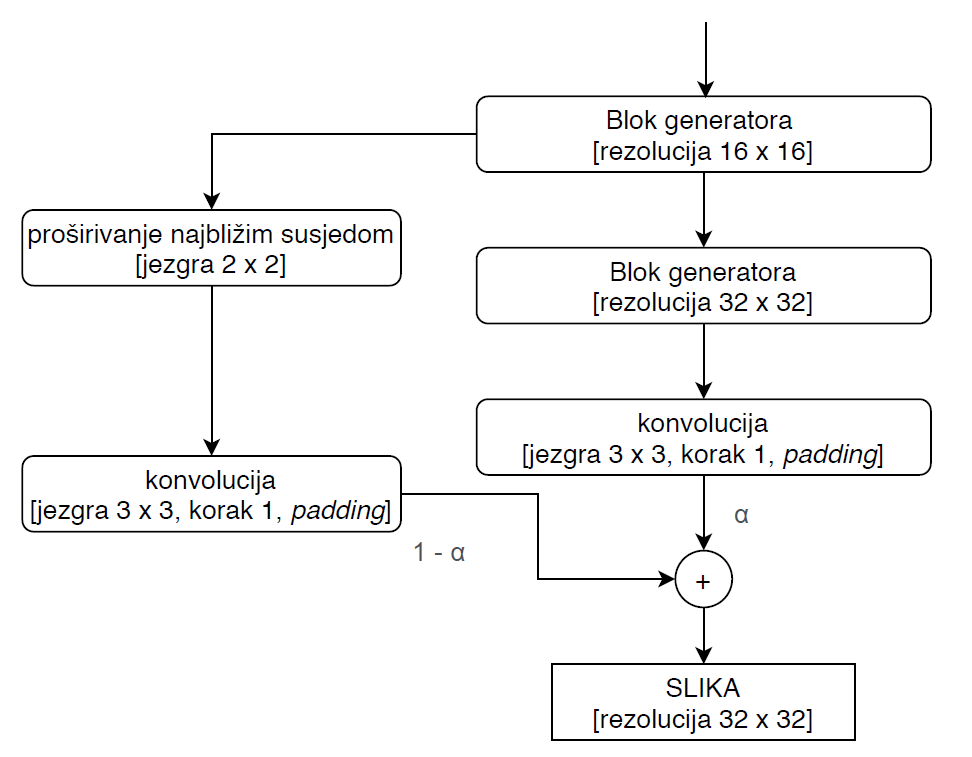
\includegraphics[height=0.7\textwidth]{images/generator_interpolation.png}
\caption{Vizualizacija interpolacije u generatoru}
\label{gen_interpolation}
\end{figure}
 
Analogno ovom postupku, odvija se i linearna interpolacija između ulaza u diskriminatoru (slika \ref{disc_interpolation}). 

\begin{figure}[h]
\centering
		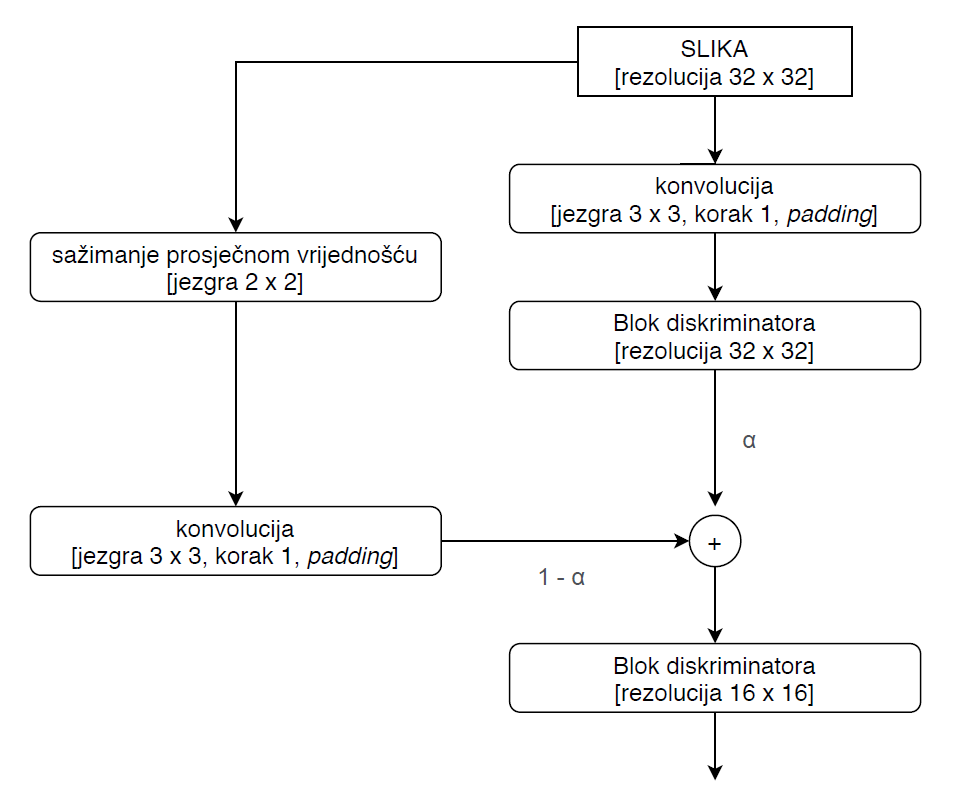
\includegraphics[height=0.7\textwidth]{images/discriminator_interpolation.png}
\caption{Vizualizacija interpolacije u diskriminatoru}
\label{disc_interpolation}
\end{figure}

Faza stabilizacije traje dok mrežama nije predočeno ukupno 800 000 stvarnih slika, odnosno 4 epohe.

Zatim nastupa faza učenja u kojoj zanemarujemo izlaz niže rezolucije, nego učimo samo pomoću više rezolucije. Kao i stabilizacija, ova faza traje dok ne predočimo 800 000 slika. Napominjemo još jednom da se uče i parametri nižih slojeva, odnosno ne zamrzavaju se.

Zbog ograničenih hardverskih mogućnosti, trenirali smo samo do rezolucije $64 \times 64$. Nakon što smo istrenirali model od najniže rezolucije do ciljne, odredili smo u kojem je trenutku treniranja model proizvodio vizualno najprihvatljivije rezultate te ponovno započeli treniranje koristeći postojeće težine kao početne, uz smanjenu stopu učenja. 

Generativna suparnička mreža istrenirana je koristeći jedan Tesla V100 GPU od 16 GB. Početna faza treniranja trajala je 30 h, od čega je 16 h na najvišoj rezoluciji te dodatnih 16 h pri rafiniranju parametara mreže. 

Korišteni hiperparametri nalaze se u tablici \ref{tablica_hiper}.

\begin{table}[h]
\caption{Korišteni hiperparametri}
\begin{center}
\begin{tabular}{|c|c|} 
 \hline
 Veličina minigrupe & 16\\ 
 \hline
 Veličina ulaznog slučajnog vektora & 512\\
 \hline
 Stopa učenja generatora & 0.001\\ 
 \hline
 Stopa učenja diskriminatora & 0.001\\ 
 \hline
 Veličina skupa za treniranje & 200000\\
 \hline
 Broj stabilizacijskih epoha & 4\\
 \hline
 Broj epoha učenja & 4\\
 \hline
 Parametar propusne zglobnice & 0.2\\
 \hline
 Parametar gradijentne kazne & 10\\
 \hline
\end{tabular}
\end{center}
\label{tablica_hiper}
\end{table}